\documentclass{ximera}

%\usepackage{todonotes}

\newcommand{\todo}{}

\usepackage{tkz-euclide}
\tikzset{>=stealth} %% cool arrow head
\tikzset{shorten <>/.style={ shorten >=#1, shorten <=#1 } } %% allows shorter vectors

\usepackage{tkz-tab}  %% sign charts
\usetikzlibrary{decorations.pathreplacing} 

\usetikzlibrary{backgrounds} %% for boxes around graphs
\usetikzlibrary{shapes,positioning}  %% Clouds and stars
\usetikzlibrary{matrix} %% for matrix
\usepgfplotslibrary{polar} %% for polar plots
\usetkzobj{all}
\usepackage[makeroom]{cancel} %% for strike outs
%\usepackage{mathtools} %% for pretty underbrace % Breaks Ximera
\usepackage{multicol}

\usepackage{polynom}



\usepackage[many]{tcolorbox}  %% for titled boxes
\newtcolorbox{xbox}[1]{%
    tikznode boxed title,
    enhanced,
    arc=0mm,
    interior style={white},
    attach boxed title to top center= {yshift=-\tcboxedtitleheight/2},
    fonttitle=\bfseries,
    colbacktitle=white,coltitle=black,
    boxed title style={size=normal,colframe=white,boxrule=0pt},
    title={#1}}


\usepackage{array}
\setlength{\extrarowheight}{+.1cm}   
\newdimen\digitwidth
\settowidth\digitwidth{9}
\def\divrule#1#2{
\noalign{\moveright#1\digitwidth
\vbox{\hrule width#2\digitwidth}}}





\newcommand{\RR}{\mathbb R}
\newcommand{\R}{\mathbb R}
\newcommand{\N}{\mathbb N}
\newcommand{\Z}{\mathbb Z}

%\renewcommand{\d}{\,d\!}
\renewcommand{\d}{\mathop{}\!d}
\newcommand{\dd}[2][]{\frac{\d #1}{\d #2}}
\newcommand{\pp}[2][]{\frac{\partial #1}{\partial #2}}
\renewcommand{\l}{\ell}
\newcommand{\ddx}{\frac{d}{\d x}}
\newcommand{\ddt}{\frac{d}{\d t}}

\newcommand{\zeroOverZero}{\ensuremath{\boldsymbol{\tfrac{0}{0}}}}
\newcommand{\inftyOverInfty}{\ensuremath{\boldsymbol{\tfrac{\infty}{\infty}}}}
\newcommand{\zeroOverInfty}{\ensuremath{\boldsymbol{\tfrac{0}{\infty}}}}
\newcommand{\zeroTimesInfty}{\ensuremath{\small\boldsymbol{0\cdot \infty}}}
\newcommand{\inftyMinusInfty}{\ensuremath{\small\boldsymbol{\infty - \infty}}}
\newcommand{\oneToInfty}{\ensuremath{\boldsymbol{1^\infty}}}
\newcommand{\zeroToZero}{\ensuremath{\boldsymbol{0^0}}}
\newcommand{\inftyToZero}{\ensuremath{\boldsymbol{\infty^0}}}



\newcommand{\numOverZero}{\ensuremath{\boldsymbol{\tfrac{\#}{0}}}}
\newcommand{\dfn}{\textbf}
%\newcommand{\unit}{\,\mathrm}
\newcommand{\unit}{\mathop{}\!\mathrm}
\newcommand{\eval}[1]{\bigg[ #1 \bigg]}
\newcommand{\seq}[1]{\left( #1 \right)}
\renewcommand{\epsilon}{\varepsilon}
\renewcommand{\iff}{\Leftrightarrow}

\DeclareMathOperator{\arccot}{arccot}
\DeclareMathOperator{\arcsec}{arcsec}
\DeclareMathOperator{\arccsc}{arccsc}
\DeclareMathOperator{\si}{Si}
\DeclareMathOperator{\proj}{proj}
\DeclareMathOperator{\scal}{scal}


\newcommand{\tightoverset}[2]{% for arrow vec
  \mathop{#2}\limits^{\vbox to -.5ex{\kern-0.75ex\hbox{$#1$}\vss}}}
\newcommand{\arrowvec}[1]{\tightoverset{\scriptstyle\rightharpoonup}{#1}}
\renewcommand{\vec}{\mathbf}
\newcommand{\veci}{\vec{i}}
\newcommand{\vecj}{\vec{j}}
\newcommand{\veck}{\vec{k}}
\newcommand{\vecl}{\boldsymbol{\l}}

\newcommand{\dotp}{\bullet}
\newcommand{\cross}{\boldsymbol\times}
\newcommand{\grad}{\boldsymbol\nabla}
\newcommand{\divergence}{\grad\dotp}
\newcommand{\curl}{\grad\cross}
%\DeclareMathOperator{\divergence}{divergence}
%\DeclareMathOperator{\curl}[1]{\grad\cross #1}


\colorlet{textColor}{black} 
\colorlet{background}{white}
\colorlet{penColor}{blue!50!black} % Color of a curve in a plot
\colorlet{penColor2}{red!50!black}% Color of a curve in a plot
\colorlet{penColor3}{red!50!blue} % Color of a curve in a plot
\colorlet{penColor4}{green!50!black} % Color of a curve in a plot
\colorlet{penColor5}{orange!80!black} % Color of a curve in a plot
\colorlet{fill1}{penColor!20} % Color of fill in a plot
\colorlet{fill2}{penColor2!20} % Color of fill in a plot
\colorlet{fillp}{fill1} % Color of positive area
\colorlet{filln}{penColor2!20} % Color of negative area
\colorlet{fill3}{penColor3!20} % Fill
\colorlet{fill4}{penColor4!20} % Fill
\colorlet{fill5}{penColor5!20} % Fill
\colorlet{gridColor}{gray!50} % Color of grid in a plot

\newcommand{\surfaceColor}{violet}
\newcommand{\surfaceColorTwo}{redyellow}
\newcommand{\sliceColor}{greenyellow}




\pgfmathdeclarefunction{gauss}{2}{% gives gaussian
  \pgfmathparse{1/(#2*sqrt(2*pi))*exp(-((x-#1)^2)/(2*#2^2))}%
}


%%%%%%%%%%%%%
%% Vectors
%%%%%%%%%%%%%

%% Simple horiz vectors
\renewcommand{\vector}[1]{\left\langle #1\right\rangle}


%% %% Complex Horiz Vectors with angle brackets
%% \makeatletter
%% \renewcommand{\vector}[2][ , ]{\left\langle%
%%   \def\nextitem{\def\nextitem{#1}}%
%%   \@for \el:=#2\do{\nextitem\el}\right\rangle%
%% }
%% \makeatother

%% %% Vertical Vectors
%% \def\vector#1{\begin{bmatrix}\vecListA#1,,\end{bmatrix}}
%% \def\vecListA#1,{\if,#1,\else #1\cr \expandafter \vecListA \fi}

%%%%%%%%%%%%%
%% End of vectors
%%%%%%%%%%%%%

%\newcommand{\fullwidth}{}
%\newcommand{\normalwidth}{}



%% makes a snazzy t-chart for evaluating functions
%\newenvironment{tchart}{\rowcolors{2}{}{background!90!textColor}\array}{\endarray}

%%This is to help with formatting on future title pages.
\newenvironment{sectionOutcomes}{}{} 



%% Flowchart stuff
%\tikzstyle{startstop} = [rectangle, rounded corners, minimum width=3cm, minimum height=1cm,text centered, draw=black]
%\tikzstyle{question} = [rectangle, minimum width=3cm, minimum height=1cm, text centered, draw=black]
%\tikzstyle{decision} = [trapezium, trapezium left angle=70, trapezium right angle=110, minimum width=3cm, minimum height=1cm, text centered, draw=black]
%\tikzstyle{question} = [rectangle, rounded corners, minimum width=3cm, minimum height=1cm,text centered, draw=black]
%\tikzstyle{process} = [rectangle, minimum width=3cm, minimum height=1cm, text centered, draw=black]
%\tikzstyle{decision} = [trapezium, trapezium left angle=70, trapezium right angle=110, minimum width=3cm, minimum height=1cm, text centered, draw=black]


\author{Nela Lakos \and Bart Snapp}

\outcome{Identify situations where logs can be used to help find derivatives.}
\outcome{Use logarithmic differentiation to simplify taking derivatives.}
\outcome{Take derivatives of logarithms and exponents of all bases.}
\outcome{Take derivatives of functions raised to functions.}
\outcome{Recognize the difference between a variable as the base and a variable as the exponent.}
\outcome{Work with the inverse properties of functions.}

\title[Dig-In:]{Logarithmic differentiation}

\begin{document}
	\begin{abstract}
		We use logarithms to help us differentiate.
	\end{abstract}
	\maketitle
	
	Logarithms were originally developed as a computational tool. The key
	fact that made this possible is that:
	\[
	\log_b(xy) = \log_b(x)+\log_b(y).
	\]
	\begin{image}
		\begin{tikzpicture}
		\begin{axis}[
		xmin=-1,xmax=7,ymin=-4,ymax=3.5,
		axis lines=center,
		xlabel=$x$, ylabel=$y$,
		every axis y label/.style={at=(current axis.above origin),anchor=south},
		every axis x label/.style={at=(current axis.right of origin),anchor=west},
		xtick={1,...,7},
		]        
		\addplot [very thick, penColor, samples=100, smooth, domain=(.01:7)] {ln(x)};
		\addplot [very thick, penColor4] plot coordinates {(2,0) (2,.693)};
		\addplot [very thick, penColor5] plot coordinates {(3,0) (3,1.099)};
		\addplot [very thick, penColor4] plot coordinates {(6,0) (6,.693)};
		\addplot [very thick, penColor5] plot coordinates {(6,.693) (6,1.792)};
		\end{axis}
		\end{tikzpicture}
		%% \caption{A plot of $\ln(x)$. Here we see that \[\ln(2\cdot 3) = \ln(2) + \ln(3).\]}
		%% \label{plot:ln additive property}
	\end{image}
	
	Before the days of calculators and computers, this was critical
	knowledge for anyone in a computational discipline.
	
	\begin{example}
		Compute $138\cdot 23.4$ using logarithms.
		\begin{explanation}
			Start by writing both numbers in scientific notation
			\[
			\left(1.38\cdot 10^{\answer[given]{2}}\right)\cdot \left(2.34 \cdot 10^{\answer[given]{1}}\right).
			\]
			Next we use a log-table, which gives $\log_{10}(N)$ for values of
			$N$ ranging between $0$ and $9$. We've reproduced part of such a
			table below.
			\begin{image}
				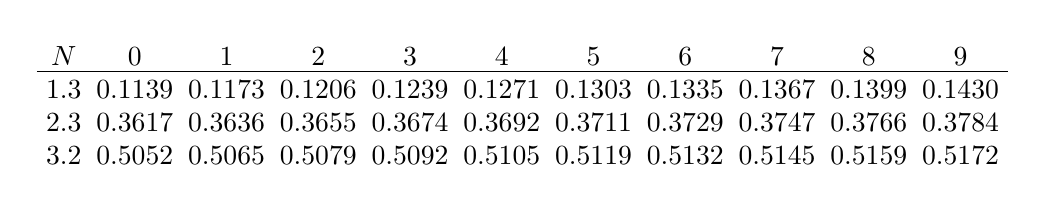
\begin{tikzpicture}
				\matrix (m) [matrix of math nodes, row sep=-.3ex, column sep=-.3ex,ampersand replacement=\&]
				{N \& 0 \& 1 \& 2 \& 3 \& 4 \& 5 \& 6 \& 7 \& 8 \& 9 \\ \hline
					1.3 \& 0.1139 \& 0.1173 \& 0.1206 \& 0.1239 \& 0.1271 \& 0.1303 \& 0.1335 \& 0.1367 \& 0.1399 \& 0.1430 \\
					%\hdotsfor{11} \\ 
					2.3 \& 0.3617 \& 0.3636 \& 0.3655 \& 0.3674 \& 0.3692 \& 0.3711 \& 0.3729 \& 0.3747 \& 0.3766 \& 0.3784 \\
					%\hdotsfor{11} \\
					3.2 \& 0.5052 \& 0.5065 \& 0.5079 \& 0.5092 \& 0.5105 \& 0.5119 \& 0.5132 \& 0.5145 \& 0.5159 \& 0.5172\\};
				\end{tikzpicture}
			\end{image}
			From the table, we see that 
			\[
			\log_{10}(1.38) \approx \answer[given]{0.1399}\qquad\text{and}\qquad \log_{10}(2.34)\approx \answer[given]{0.3692}
			\]
			Add these numbers together to get $\answer[given]{0.5091}$.
			Essentially, we know the following at this point:
			\begin{center}
				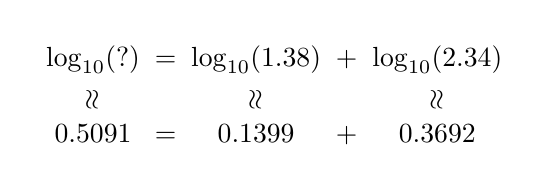
\begin{tikzpicture}
				\matrix (m) [matrix of math nodes, row sep=-.3ex, column sep=-.3ex,ampersand replacement=\&]
				{\log_{10}(\mathrm{?}) \& = \& \log_{10}(1.38) \& + \& \log_{10}(2.34)\\
					\rotatebox[origin=c]{90}{$\approx$}  \& \& \rotatebox[origin=c]{90}{$\approx$}   \& \& \rotatebox[origin=c]{90}{$\approx$}  \\
					0.5091 \& = \& 0.1399 \& + \& 0.3692\\};
				\end{tikzpicture}
			\end{center}
			Using the table again, we see that
			$\log_{10}(\answer[given]{3.23})\approx 0.5091$. Since we were
			working in scientific notation, we need to multiply this by
			$10^3$. Our final answer is
			\[
			3230 \approx 138\cdot 23.4
			\]
			Since $138\cdot 23.4 = 3229.2$, this is a good approximation.
		\end{explanation}
	\end{example}
	The moral is:
	\begin{quote}
		\textbf{Logarithms allow us to use addition in place of multiplication.}
	\end{quote}
	
	
	\section{Logarithmic differentiation}
	
	
	When taking derivatives, both the product rule and the quotient rule
	can be cumbersome to use. Logarithms will save the day. A key point is
	the following
	\[
	\ddx \ln(f(x)) = \frac{1}{f(x)}\cdot f'(x) = \frac{f'(x)}{f(x)}
	\]
	which follows from the chain rule. Let's look at an illustrative
	example to see how this is actually used.
	
	\begin{example} 
		Compute:
		\[
		\ddx \frac{x^9e^{4x}}{\sqrt{x-4}}
		\]
		\begin{explanation}
			Recall the properties of logarithms:
			\begin{itemize}
				\item $\log_b(xy) = \log_b(x) + \log_b(y)$
				\item $\log_b(x/y) = \log_b(x) - \log_b(y)$
				\item $\log_b(x^y) = y\log_b(x)$
			\end{itemize}
			
			While we could use the product and quotient rule to solve this
			problem, it would be tedious. Start by taking the logarithm of the
			function to be differentiated.
			\begin{align*}
				\ln\left(\frac{x^9e^{4x}}{\sqrt{x-4}} \right) &= \ln\left(\answer[given]{x^9e^{4x}}\right) - \ln\left(\answer[given]{\sqrt{x-4}}\right)\\
				&= \ln\left(x^9\right)+\ln\left(e^{4x}\right) - \ln\left((x-4)^{1/2}\right)\\
				&= \answer[given]{9}\ln(x)+4x - \answer[given]{\frac{1}{2}}\ln(x-4).
			\end{align*}
			Setting $f(x) = \frac{x^9e^{4x}}{\sqrt{x-4}}$, we can write
			\[
			\ln(f(x)) = 9\ln(x)+4x - \frac{1}{2}\ln(x-4).
			\]
			Differentiating both sides, we find
			\[
			\frac{f'(x)}{f(x)} = \answer[given]{\frac{9}{x}+4} - \frac{1}{2(x-4)}.
			\]
			Finally we solve for $f'(x)$, write
			\[
			f'(x) = \left(\frac{9}{x}+4 - \frac{1}{2(x-4)}\right)\left(\answer[given]{\frac{x^9e^{4x}}{\sqrt{x-4}}}\right).
			\]
		\end{explanation}
	\end{example}
	
	The process above is called \textit{logarithmic
		differentiation}. Logarithmic differentiation allows us to compute
	new derivatives too.
	
	\begin{example}
		For  $x>0$, compute 
		\[
		\ddx x^x
		\]
		\begin{explanation}
			The function $x^x$ is tricky to differentiate. We cannot use the power
			rule, as the exponent is not a constant; the function is not an exponential function either, since the base is not a constant. However, if we set $f(x) =
			x^x$ we can write
			\begin{align*}
				\ln(f(x)) &= \ln\left(x^x\right)\\
				&=x\ln(x).
			\end{align*}
			Differentiating both sides, we find
			\[
			\frac{f'(x)}{f(x)} = \answer[given]{1 + \ln(x)}.
			\]
			Now we can solve for $f'(x)$, 
			\[
			f'(x) = x^x + x^x\ln(x).
			\]
		\end{explanation}
	\end{example}
	
	
	\begin{example}
		%\author{Nela Lakos}
		Compute the derivative.
		\[
		\ddx\ln{(|x|)}
		\]
		\begin{explanation}
			The function $|x|$ is a piecewise defined function.  If $x>0$
			\begin{align*}
				\ddx\ln{(|x|)} &= \ddx\ln{(\answer[given]{x})}\\
				&=\frac{1}{\answer[given]{x}}.
			\end{align*}
			The function $\ln{(|x|)}$ is not defined at $x=0$.  If $x<0$
			\begin{align*}
				\ddx\ln{(|x|)} &= \ddx\ln{(\answer[given]{-x})}\\
				&=\frac{-1}{\answer[given]{-x}}\\
				&=\answer[given]{\frac{1}{x}}.
			\end{align*}
		\end{explanation}
	\end{example}
	
	The next  example will be useful when we want to use logarithmic differentiations for functions that  assume negative values. 
	
	
	\begin{example}
		%\author{Nela Lakos}
		Compute the derivative.
		\[
		\ddx\ln{(|f(x)|)}
		\]
		\begin{explanation}
			By the previous example and the Chain Rule
			\begin{align*}
				\ddx\ln{(|f(x)|)} &=\answer[given]{\frac{1}{f(x)}}\cdot f'(x).\\
				&=\frac{f'(x)}{\answer[given]{f(x)}}
			\end{align*}
		\end{explanation}
	\end{example}
	
	
	\section{Proof of the power rule}
	
	
	Finally, recall that previously we only proved the power rule for
	positive integer exponents. Now we'll use logarithmic differentiation to give
	a proof for all real-valued exponents. We restate the power rule
	for convenience sake:
	
	\begin{theorem}[Power Rule]\index{power rule}
		For any  real number $n$, 
		\[
		\ddx x^n = n x^{n-1}.
		\]
		\begin{explanation}
			
			We will use logarithmic differentiation. Set $f(x) = x^n$. Write
			\begin{align*}
				\ln(|f(x)|) &= \ln\left(|x|^n\right) , x\ne0\\ 
				&= n\ln(|x|).
			\end{align*}
			Now differentiate both sides, and solve for $f'(x)$
			\begin{align*}
				\frac{f'(x)}{f(x)} &= \frac{n}{x}\\
				f'(x) &=\frac{n f(x)}{x}\\
				&= \answer[given]{n x^{n-1}}.
			\end{align*}
			Whenever $x=0$ is in the domain of $f$, the definition of the derivative at $x=0$ implies that  $f'(0)=0$, if $n\ne1$ and $f'(0)=1$, if $n=1$ , so the power rule applies to $x=0$, too.\\
			
			Thus we see that the power rule holds for all real-valued (nonzero) exponents.
		\end{explanation}
	\end{theorem}
	
	While logarithmic differentiation might seem strange and new at
	first, with a little practice it will seem much more natural to you.
	
\end{document}
